\chapter{Stand der Wissenschaft und Auswahl von Verfahren}

\label{cha_state}

In diesem Kapitel soll der aktuelle Stand der Forschung und Entwicklung bezogen auf die in dieser Arbeit verwendeten Klassen von Systemen bzw. Verfahren betrachtet sowie ausgehend von den Anforderungen an das zu entwickelnde System passende Lösungen ausgewählt und in für folgende Kapitel notwendiger Detailtiefe beschrieben werden. 

Der erste Abschnitt befasst sich mit zum Zeitpunkt der Erstellung dieser Arbeit verfügbaren SIEM-Systemen und beschreibt Eigenschaften des ausgewählten Systems näher, die für die Integration des in dieser Arbeit zu entwickelnden Prototypen relevant sind.

Im zweiten Abschnitt werden Eigenschaften von Pseudonymen und Anforderungen an die Verwendung von Pseudonymisierung herausgearbeitet, die bei der Entwicklung eines Systems beachtet werden müssen.

Der dritte Abschnitt stellt den Forschungsstand im Bereich der kryptographischen Schwellwertschemata dar und beschreibt das ausgewählte Verfahren im Detail.

Der letzte Abschnitt befasst sich mit verschiedenen Ansätzen zur Lösung des in Abschnitt \ref{TODO} dargelegten Problems des Wiederverwendens bereits vergebener Pseudonyme für ein eintreffendes Datum inklusive möglicher Vor- und Nachteile und trifft darauf basierend eine Auswahl für ein zu implementierendes Verfahren. 

\section{SIEM-Systeme}

\label{sec_state_siem}

Zur Zeit gibt es eine vielfältige Auswahl an SIEM-Systemen auf dem Markt: Splunk\footnote{
  https://www.splunk.com
}, QRadar von IBM\footnote{
  https://www.ibm.com/us-en/marketplace/ibm-qradar-siem
} oder ArcSight von Micro Focus\footnote{
  https://software.microfocus.com/en-us/software/siem-security-information-event-management
} sind nur einige Beispiele aus diesem Bereich. Neben den in Abschnitt \ref{sec_basics_siem} beschriebenen grundlegenden Funktionen eines SIEM-Systems, die von allen Kandidaten in unterschiedlichem Maße bereitgestellt werden, unterscheiden sie sich insbesondere in darüber hinausgehenden Techniken: Die Nutzung von Machine Learning zur Erkennung ungewöhnlichem Verhaltens oder die Automatisierung von Handlungen im Bedrohungsfall sind hier beispielhafte Möglichkeiten.

Die Auswahl an quelloffener Software in diesem Bereich ist jedoch sehr gering. Eine Ausnahme stellt OSSIM - ein SIEM-System der Firma AlienVault\footnote{
	AlienVault OSSIM: The World’s Most Widely Used Open Source SIEM\\https://www.alienvault.com/products/ossim
} - dar, das auf Basis weiterer quelloffener Lösungen aus dem Netzwerksicherheits-Bereich unter anderem die in Abschnitt \ref{sec_basics_siem} beschriebenen Funktionen bereitstellt. AlienVault bietet zusätzliche eine kommerzielle Variante seines Produkts namens USM an, das insbesondere in den Bereichen Event-Korrelation und Compliance-Reporting die Funktionalität von OSSIM übersteigt. Von der Entwicklungsarbeit die in USM fließt, profitiert jedoch auch OSSIM, beispielsweise durch die Aktualisierung von Plugins für die Einbindung von aktuellen Netzwerkgeräten.

Da die Quelloffenheit auch die Möglichkeit bietet, Komponenten des SIEM-Systems direkt zu verändern, und außerdem gerade im Sicherheitsbereich generell zu bevorzugen ist, fiel die Entscheidung des in dieser Arbeit verwendeten SIEM-Systems auf OSSIM.

\subsection{OSSIM-Überblick}

\label{subsec_state_siem_overview}

Im Folgenden soll eine Übersicht über die für diese Arbeit relevanten Komponenten von OSSIM und deren Zusammenspiel gegeben werden. Diese ist auch in Abbildung \ref{fig:ossim_log_flow} dargestellt.

Den Kern des SIEM-Systems bildet der OSSIM-Server. Hier werden Events gespeichert sowie aggregiert und es findet die Korrelation von Events statt, die der Erkennung von Angriffen oder ungewöhnlichem Netzverhalten dient. Events und generierte Meldungen können über ein Web Interface betrachtet werden. Weiterhin können hier unter anderem Angaben zur Netzinfrastruktur bereitgestellt, Netzwerk- und Schwachstellenscanner bedient und sämtliche Informationen über den Netzwerkstatus eingesehen werden. 

Der OSSIM-Agent ist dafür zuständig, vorliegende Logdaten zu parsen und in ein OSSIM-spezifisches Event-Format zu übersetzen. Auf diesen Vorgang wird im nächsten Abschnitt genauer eingegangen. Die erzeugten Events werden anschließend an den Server weitergeleitet. Der Agent befindet sich sowohl direkt auf dem Server als auch auf jedem installierten Sensor. 

Eine OSSIM-Umgebung kann optional ein oder mehrere Sensoren nutzen, auf denen jeweils ein Agent seine Arbeit verrichtet. Dies wird im Folgenden verteilte Installation genannt. Der Vorteil dieser Lösung besteht darin, dass das aufwendige Parsen und Normalisieren von Logdaten verteilt staffinden und dadurch die Serverlast in großen Umgebungen reduziert werden kann. Kommt kein externer Sensor zum Einsatz, so spricht man von einer All-In-One-Installation.

\begin{figure}[]
    \centering
        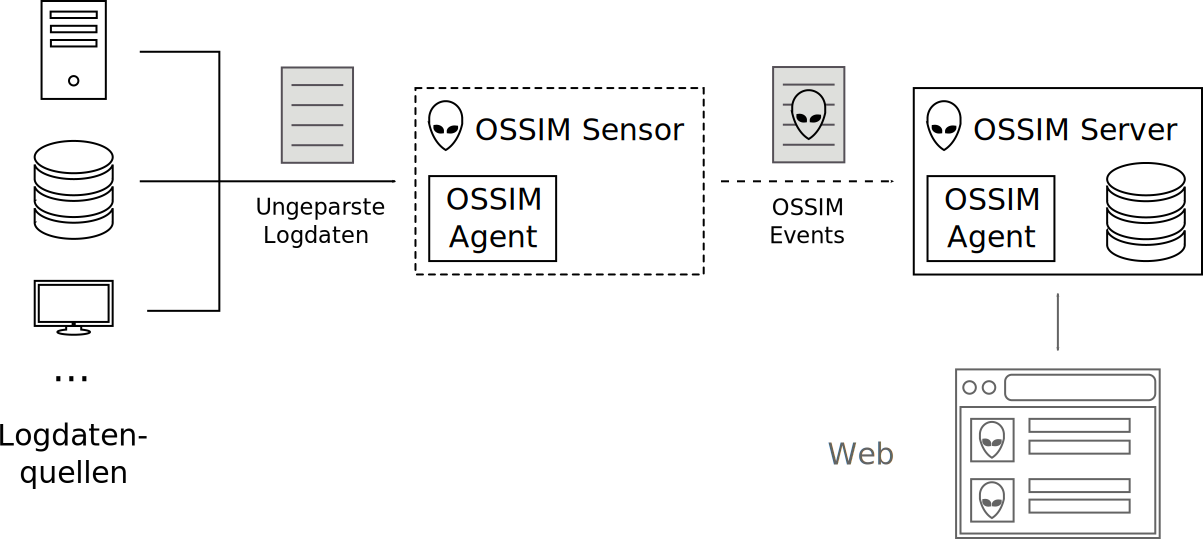
\includegraphics[width=0.9\textwidth]{dia/ossim_log_flow.pdf}
    \caption{High-Level-Übersicht über die OSSIM-Architektur und den Datenfluss.}
    \label{fig:ossim_log_flow}
\end{figure}


\subsection{Parsen von Logdaten in OSSIM}

\label{subsec_state_siem_parsing}

% Quellenarten
% Plugins
% OSSIM-Events
Besonders von Bedeutung für diese Arbeit ist die Verarbeitung von Logdaten. OSSIM ermöglicht es, Logdaten aus unterschiedlichen Quellen entgegenzunehmen bzw. aktiv selber abzurufen und in ein gemeinsames Event-Format zu übersetzen. Hierzu stehen verschiedene Möglichkeiten zur Verfügung:

\begin{itemize}
  \item Entgegennehmen von Daten über das Syslog-Protokoll
  \item Beschaffen von Daten über das SNMP-Protokoll
  \item Entgegennehmen von Daten über proprietäre Protokoll wie SDEE oder WMI
  \item Beschaffen von Daten durch Datenbankabfragen 
\end{itemize}

Unabhängig von der Datenquelle funktioniert die Verarbeitung der Logdaten nach dem immer gleichen Schema. OSSIM bietet die Möglichkeit mitgelieferte oder selber entwickelte Plugins für verschiedene Datenquellen zu aktivieren. Für eintreffende Logdaten überprüft der Agent anhand von regulären Audrücken, ob ein Plugin für das entsprechende Datum zuständig ist. Ist so ein Plugin gefunden, so wird ein neues OSSIM-Event angelegt und anhand der Angaben im Plugin die entsprechenden vorgegebenen Felder des Events gesetzt. Hierbei kann es sich beispielsweise um den Zeitpunkt des Events, IP-Adresse und Port der Datenquelle, einen zu dem Event gehörigen Netzwerkbenutzer oder ereignisabhängige selbstgesetzte Felder handeln. Anschließend folgt die Weiterleitung des Events an den Server.


\section{Pseudonymisierung}

\label{sec_state_pseudonymity}

- A name or another bit string. Identifiers, which are generated using random data only, i.e., fully 
independent of the subject and related attribute values, do not contain side information on the 
subject they are attached to, whereas non-random identifiers may do. E.g., nicknames chosen by 
a user may contain information on heroes he admires; a sequence number may contain 
information on the time the pseudonym was issued; an e-mail address or phone number contains 
information how to reach the user.  \cite{pfitzmann2010}

- evtl. Common Criteria

- VANET

- TIMSI

%pfitzmann2001 - Abschnitt 12
Der Begriff der Pseudonymisierung beschreibt die Benutzung von Pseudonymen zur Identifizierung von Subjekten. Pseudonymisierung sagt dabei erst einmal lediglich etwas über die Verwendung eines Verfahrens aus, jedoch nichts über die daraus entstehenden Auswirkungen auf die Identifizierbarkeit eines Subjekts oder die Zurechenbarkeit bestimmter Aktionen. Hierfür spielen weitere Eigenschaften von Pseudonymen wie die folgenden eine Rolle:
\begin{itemize}
  \item garantierte Eindeutigkeit von Pseudonymen
  \item Möglichkeit von Pseudonymänderungen
  \item begrenzt häufige Verwendung von Pseudonymen 
  \item zeitlich begrenzte Verwendung von Pseudonymen
  \item Art der Pseudonymserstellung
\end{itemize}

Die Ausprägungen dieser Eigenschaften werden auch im Rahmen dieser Arbeit für das umzusetzende System zu bewerten sein.

\section{Schwellwertschemata}

\begin{itemize}
  \item \textbf{Grundlagen} Von Shamirs Secret Sharing bis heute
  \item \textbf{Konkretes Verfahren} Im Detail erläutern - vmtl. Desmedt auf Basis von ElGamal
  \item Zusätzlich Erweiterungen dieses Verfahrens wie verteilte Schlüsselgenerierung.
\end{itemize}

%- Desmedt, Frankel: ElGamal \cite{DesmedtFrankel1990}
%- setzt zentralen "Dealer" voraus
%- Pedersen und verbesserte Variante 
%- Andere Möglichkeiten: Paillier, RSA, ...

\label{sec_state_threshold}

Ein solches System, das auf dem ElGamal-Algorithmus und damit dem Diskreten-Logarithmus-Problem basiert, veröffentlichten die Autoren in \cite{DesmedtFrankel1990}. \todo{Details} Dieser Ansatz setzt in der \textit{Setup}-Phase auf eine zentrale vertrauenswürdige Stelle zur Erzeugung der Schlüssel und \textit{Shares}. In \cite{pedersen1991} stellt der Autor basierend auf diesen Ergebnissen ein Verfahren vor, das bei der Schlüsselgenerierung ohne eine vertrauenswürdige Instanz auskommt. Dieses Verfahren wird in \cite{gennaro1999} noch einmal verbessert.\\
Basierend auf dem jetzigen Recherchestand würde sich diese Kombination von Verfahren gut für den angestrebten Anwendungszweck eignen. Konkrete offene Implementierungen wurden jedoch bisher nicht gefunden, so dass möglicherweise eine eigene Implementierung umgesetzt werden muss.

Neben diesem Verfahren gibt es noch weitere Ansätze basierend auf RSA \cite{desmedt1993, nguyen2005} oder dem Paillier-Kryptosystem \cite{paillier1999, damgard2001}, die jedoch deutlich komplexer zu sein scheinen. 

\todo{TBW}

\section{Searchable Encryption}

\label{sec_state_se}

%- Problemstellung: wie herausfinden, ob für ein Datum bereits ein Pseudonym vorliegt, obwohl die Daten lediglich nicht entschlüsselbar vorliegen? Außerdem auch Notwendigkeit des  Nicht-Determinismus für Searchable Encryption erwähnen (Public Key Verfahren).
%
%- Lösungsmöglichkeiten aufbauend jeweils mit Bewertung der Möglichkeit:
%  - Entschlüsseln und überprüfen: nicht möglich durch threshold, außerdem performance
%  - Local Mapping
%  - Einfacher Hash: Bruteforce bei kleinem Werteraum einfach (bspw. Mitarbeiternamen)
%  - Searchable Encryption (siehe Grundlagen)
%    - MAC als einfachste Form deterministischer Verschlüsselung
%    - Andere Formen...
%    
%- Mögliche Bewertungskriterien:
%  - Was muss abgesichert werden und wo muss es vorliegen?
%  - Mehrere Suchworte zu einem Pseudonym möglich? (zB Name, IP, ... ) Gewünscht? Welche Vorteile könnte dies beispielsweise bezogen auf den Anwendungsfall der Insidererkennung bringen?
%  - Verteilte Pseudonymhaltung möglich? Was müsste verteilt werden?


\todo{Problematik bereits in Übersichtskapitel darstellen -> auslagern?}

Trifft ein neues Datum in dem System ein und soll pseudonymisiert werden, so muss überprüft werden, ob bereits ein Pseudonym für das Datum vergeben wurde. 
Da die Daten jedoch in  verschlüsselter Form vorliegen, stellt sich die Frage, wie diese Überprüfung erreicht werden kann. In Abbildung \ref{fig:se_overview} ist dieses Problem noch einmal anhand eines Beispiels dargestellt. Zu einem Zeitpunkt liegen in der Pseudonymtabelle Pseudonyme für zwei Benutzer \textit{User A} und \textit{User B} vor. Das diese Benutzer zu den Pseudonymen gehören, ist jedoch nicht offensichtlich, da die Daten verschlüsselt gespeichert sind. Sollen nun neue Logdaten verarbeitet werden, liegen zwei mögliche Fälle vor: 

\begin{itemize}
  \item Es liegt bereits ein Pseudonym für den Benutzer vor (linker Bereich in der Darstellung). Hier muss das bereits vergebene Pseudonym \textit{0x1301} verwendet werden.
  \item Es liegt noch kein Pseudonym für den Benutzer vor (rechter Bereich in der Darstellung). Nun wird ein neues Pseudonym \textit{0x805A} angelegt und verwendet werden.
\end{itemize}

Verschiedene Lösungmöglichkeiten inklusive ihrer Vor- und Nachteile für das Problem, wie nun trotz der Verschlüsselung der Daten dieses Verhalten erreicht werden kann, werden in diesem Abschnitt beleuchtet.

\begin{figure}[]
    \centering
        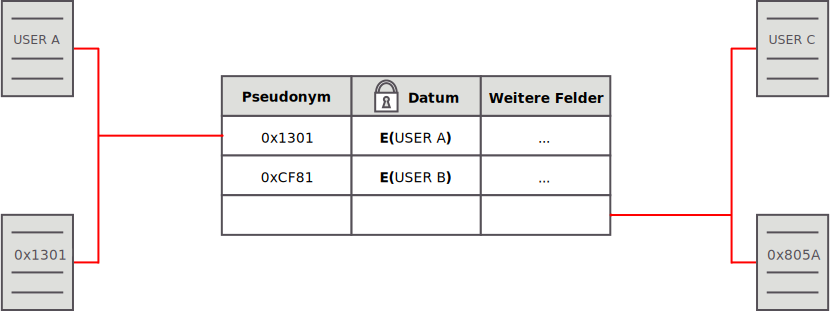
\includegraphics[width=0.9\textwidth]{dia/se_overview.pdf}
    \caption{Erhalt von Pseudonymen aus der Zuordnungstabelle: Links für den Fall eines bereits bekannten Datums (hier Benutzer), rechts für ein unbekanntes Datum.}
    \label{fig:se_overview}
\end{figure}

\subsection{Entschlüsseln aller Datensätze}

Da für die Verschlüsselung ein kryptographisches Schwellwertschema verwendet wird, scheiden zwei triviale Möglichkeiten aus: Das Entschlüsseln aller Datensätze zur Überprüfung wäre nicht nur unter Performance-Gesichtspunkten nicht wünschenswert. Es darf auch nicht möglich sein, da die \textit{Shares} zur Entschlüsselung nicht am Ort der Verschlüsselung vorliegen dürfen. Dies ist eine der Grundannahmen, die der Sicherheit des Systems zugrundeliegen. 

\subsection{Deterministische Verschlüsselung}

Die zweite ausscheidende Möglichkeit wäre das Überprüfen aller Einträge auf Schlüsseltextgleichheit. Bei Gleichheit eines Eintrages könnte das entsprechende Pseudonym zurückgeliefert werden. Hierzu müsste ein deterministisches Verschlüsselungsverfahren genutzt werden, das ein Datum immer auf den gleichen Schlüsseltext abbildet. Diese Möglichkeit scheidet jedoch aus, da es sich bei dem verwendeten Schwellwertschema um ein Public-Key-Verfahren, bei dem bei der Verschlüsselung ein Zufallswert einfließt -- folglich ein nicht-deterministisches Verfahren, handelt.\\
Dieser Nicht-Determinismus ist notwendig, da ansonsten zur Aufdeckung eines Pseudonyms auch ein Wörterbuch-Angriff mithilfe des öffentlichen Schlüssels des Schwellwertschemas genutzt werden könnte. Ein Angreifer würde alle möglichen Werte, die ein Datum annehmen kann, mit dem öffentlichen Schlüssel verschlüsseln und mit dem aufzudeckenden Eintrag vergleichen. Gleichheit der Schlüsseltexte würde den gesuchten Klartext liefern. Der im Kontext dieser Arbeit vorliegende kleine und bekannte Wertebereich (wie beispielsweise Mitarbeiternamen) würde diesen Angriff relativ effizient machen. Aus diesem Grund muss ein nicht-deterministisches Verschlüsselungsverfahren genutzt werden und damit ist die Überprüfung auf Schlüsseltextgleichheit nicht möglich.


\subsection{Nutzung von Hashfunktionen}

Ein weiterer Ansatz, der ebenfalls anfällig für diese Art von Wörterbuch-Angriff wäre, ist die Verwendung von (kryptographisch sicheren) Hashfunktionen zur Suche: Neben dem Pseudonym und dem verschlüsselten Datum wird ein Hash des Datums abgespeichert. Muss nun für ein neues Datum überprüft werden, ob bereits ein Pseudonym vorliegt, kann der Hash des Datums gebildet und mit allen vorliegenden Hashes verglichen werden. Bei Übereinstimmung wäre das Datum (mit großer Wahrscheinlichkeit) gleich dem verschlüsselten Datum und das Pseudonym könnte genutzt werden. Diese Möglichkeit ist jedoch durch den bereits erwähnten kleinen Wertebereich ebenso anfällig für einen Wörterbuch-Angriff: Ein Angreifer könnte mithilfe der bekannten Hashfunktion die Hashes aller Werte berechnen und mit dem des aufzudeckenden Pseudonyms vergleichen.

\subsection{Lokale Zuordnung}

Eine andere Möglichkeit ist die Anlage einer vor externem Zugriff geschützten Zuordungstabelle zwischen Datum und Pseudonym am Ort der Ersetzung. Bei Eintreffen eines neuen Datums kann in der Tabelle das zugehörige Pseudonym ermittelt werden oder falls es noch nicht existiert, ein neues Pseudonym erstellt und zusammen mit dem verschlüsselten Datum gespeichert werden. Diese Lösung wirda auch in \cite{goh2003} erwähnt.

Nachteil bezogen auf das für diese Arbeit zu entwickelnde System ist jedoch die notwendige Generierung von Pseudonymen und Speicherung der Zuordnungstabelle an der Stelle, an der neue Daten eintreffen. Hierdurch wird ein relativ leichtgewichtiger Proxy-Server wie er in der Architektur vorhergesehen ist (siehe Abschnitt \ref{sec_impl_architecture}) verhindert. Außerdem würde eine Kompromittierung dieser Komponente direkt zur Aufdeckung des Pseudonymzusammenhanges führen. \todo{Verhindert verteiltes System - diesen Aspekt betonen (mehrere Proxies, ...)}

\subsection{Message Authentication Codes}

Aufbauend auf der Hash-basierten Lösung lässt sich jedoch auch eine nicht für einen Wörterbuch-Angriff anfällige Lösung entwickeln. Dazu wird der verwendete Hash durch einen schlüsselabhängigen Message Authentication Code (MAC) ersetzt. Beim Speichern eines neuen Eintrags wird dazu unter Zuhilfename eines zufällig generierten Schlüssels ein MAC über das Datum berechnet und mit dem Eintrag gespeichert. Für ein Datum kann jetzt durch Überprüfen aller MACs bestimmt werden, ob bereits ein Pseudonym vergeben wurde. Ein Angreifer kann den beschriebenen Wörterbuch-Angriff jedoch ohne Kenntnis des Schlüssels nicht ausführen.

Bei dieser Lösung handelt es sich um eine einfache Form der Searchable Symmetric Encryption wie sie in Abschnitt \ref{sec_basisc_se} dargestellt ist. Die durch Pseudonyme zu ersetzenden Daten bilden die zu durchsuchenden Dokumente. Der MAC bildet den Suchwort-Index für jeden verschlüsselten Eintrag und wird so auch als Trapdoor-Element für die Suche nach einem passenden Eintrag genutzt. Ausgehend von den Anforderungen des umzusetzenden Systems eignet sich dieser Ansatz: Er ermöglicht einer Komponente die Zuordnung eines Datums zu einem Pseudonym, ohne dass dass diese Zuordnung direkt gespeichert werden muss oder der Datenbank bei der Abfrage bekannt wird. Auch ein Wörterbuchangriff, der bei dem erwähnten kleinen Wertebereich geringen Aufwand bedeutete, wird verhindert. Aus diesen Gründen wird dieser Lösungsansatz in einem späteren Schritt im zu entwickelnden System umgesetzt.

Die Nutzung von deterministischer Verschlüsselung (mit der hier beschriebenen Verwendung eines MACs als Sonderfall) wird erstmals in \cite{bellare2007deterministic} beschrieben. Dort werden auch einige Schwächen dieser Lösung diskutiert: Die Datenbank erfährt durch den Suchindex bereits einiges über die gespeicherten Dokumente, da durch die deterministische Struktur gleiche Suchwörter auf gleiche Trapdoor-Elemente abgebildet werden. Diese Schwäche ist im Bezug auf den besonderen Anwendungsfall dieser Arbeit jedoch zu vernachlässigen, da Dokumente (meint Benutzernamen, ...) nur einmalig vorliegen dürfen. Eine weitere Schwäche, die auch in dieser Arbeit beachtet werden muss, ist, dass die Datenbank etwas über die Häufigkeit verschiedener Suchanfragen erfährt, da die Trapdoor-Elemente für ein bestimmtes Datum immer gleich sind. Durch Korrelation mit Hintergrundwissen könnte so möglicherweise in bestimmten Fällen der Inhaber eines Pseudonyms herausgefunden werden. 
\todo{Hash-Kollisionen und Geburtstags-Paradoxon hier erwähnen?}

\subsection{Weitere Möglichkeiten der Searchable Encryption}
\label{sec_state_se_furtherpossibilities}

%- SongWagner \cite{song2000practical}
%- survey \cite{wang2016}
%- goh \cite{goh2003}
%- chang \cite{chang2005}

Die im letzten Abschnitt betrachtete MAC-basierte Lösung funktioniert für den in dieser Arbeit behandelten Anwendungsfall. Bei der Abbildung Pseudonym zu Datum (wie den Benutzername) handelt es sich um eine 1:1-Abbildung, die lediglich von einer Komponente -- dem zu entwickelnden Syslog-Proxy \todo{Referenz auf XY?} -- abgefragt wird. 

In anderen Umgebungen bzw. Erweiterungen des in dieser Arbeit betrachteten Anwendungsfalls kann es jedoch auch andere Anforderungen geben. Vorstellbar wäre beispielsweise die verteilte Abfrage der Datenbank nach existierenden Pseudonymen. Für den MAC-basierten Ansatz müsste dazu zumindest der genutzte Schlüssel verteilt werden, was Kommunikation innerhalb der verteilten abfragenden Komponenten erfordert. Zusätzlich müssten auch die Sicherheitsauswirkungen dieser Lösung betrachtet werden.\\
Eine andere Erweiterung könnte die Mehrfachverwendung von Pseudonymen für verschiedene Merkmale eines Benutzers (Name, IP-Adresse, Signaturschlüssel, ...) sein, um die Erkennung von Insiderangriffen zu verbessern. Auch diese Erweiterung wäre mit dem MAC-basierten Ansatz nicht direkt abbildbar.

Andere Lösungsansätze für die in diesen Fällen entstehenden Probleme könnten Forschungsergebnisse aus dem Bereich der \textit{Searchable Encryption} bieten. In \cite{song2000practical} wurde von den Autoren das erste Searchable-Symmetric-Encryption-Schema entwickelt (siehe auch Abschnitt \ref{sec_basisc_se}). Verbesserte Schemata folgten in \cite{goh2003} und \cite{chang2005}. Durch diese sind variable Dokumentenlängen mit beliebig vielen Suchwörtern möglich, die auch nachträglich erweiterbar sind. Für den Aspekt der verteilten Abfrage könnten die Ergebnisse aus \cite{boneh2004public} genutzt werden, in dem sich die Autoren mit der Suche in mit asymmetrischen Verfahren verschlüsselten Daten befassen.\\
Eine Übersicht über weitere Ergebnisse in diesem Bereich lässt sich in \cite{wang2016} finden.